% SMPdesign/partexercises.tex

\section{Partitioning Exercises}
\label{sec:SMPdesign:Partitioning Exercises}

This section uses a pair of exercises (the classic Dining Philosophers
problem and a double-ended queue) to demonstrate the value of partitioning.

\subsection{Dining Philosophers Problem}
\label{sec:SMPdesign:Dining Philosophers Problem}

\begin{figure}[tb]
\begin{center}
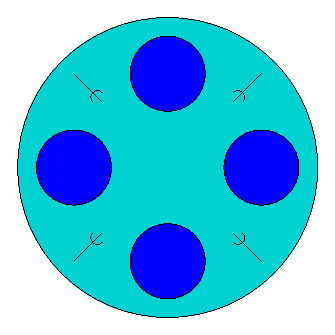
\includegraphics{SMPdesign/DiningPhilosopher4}
\end{center}
\caption{Dining Philosophers Problem}
\label{fig:SMPdesign:Dining Philosophers Problem}
\end{figure}

Figure~\ref{fig:SMPdesign:Dining Philosophers Problem} shows a diagram
of the classic Dining Philosophers problem~\cite{Dijkstra1971HOoSP}.
This problem features four philosophers who do nothing but think and
eat a ``very difficult kind of spaghetti'' which requires two forks
to eat.
A given philosopher is permitted to use only the forks to his or her
immediate right and left, and once a philosopher picks up a fork,
he or she will not put it down until sated.

The object is to construct an algorithm that, quite literally,
prevents starvation.
One starvation scenario would be if all of the philosophers picked up 
their leftmost forks simultaneously.
Because none of them would put down their fork until after they ate,
and because none of them may pick up their second fork until at least
one has finished eating, they all starve.

And, yes, Dijkstra's original formulation did in fact specify five
philosophers rather than four.
However, but 90\textsuperscript{o} angles are much
easier to work with than are 72\textsuperscript{0} angles.
This issue was presumably of less concern to Dijkstra when the
original paper appeared in 1971, during
era of typewriters and hand-drawn figures.

\begin{figure}[tb]
\begin{center}
\includegraphics{SMPdesign/DiningPhilosopher4TB}
\end{center}
\caption{Dining Philosophers Problem, Textbook Solution}
\label{fig:SMPdesign:Dining Philosophers Problem, Textbook Solution}
\end{figure}

Dijkstra's solution used a global semaphore, which works fine assuming
negligible communications delays, an assumption that has become invalid
in the ensuing decades.
Therefore, recent solutions number the forks as shown in
Figure~\ref{fig:SMPdesign:Dining Philosophers Problem, Textbook Solution}.
Each philosopher picks up the lowest-numbered fork next to his or her
plate, then picks up the highest-numbered fork.
The philosopher sitting by the uppermost plate in the diagram thus
picks up the leftmost fork first, then the rightmost fork, while the
rest of the philosophers instead pick up their rightmost fork first.
Because two of the philosophers will attempt to pick up fork~1 first,
and because only one of those two philosophers will succeed,
there will be four forks available to three philosophers.
At least one of these three will be guaranteed to have two forks,
and thus be able to proceed eating.

This general technique of numbering resources and acquiring them in
numerical order is heavily used as a deadlock-prevention technique.
However, it is easy to imagine a sequence of events that will result
in only one philosopher eating at a time even though all are hungry:

\begin{enumerate}
\item	Rightmost philosopher picks up fork~1, preventing upper philosopher
	from taking a fork.
\item	Lower philosopher picks up fork~2.
\item	Leftmost philosopher picks up fork~3.
\item	Leftmost philosopher picks up fork~4 and eats.
\item	Leftmost philosopher puts down forks~3 and 4.
\item	Lower philosopher picks up fork~3 and eats.
\end{enumerate}

Please think about ways of partitioning the Dining Philosophers Problem
before reading further.
\clearpage


\begin{figure}[tb]
\begin{center}
\includegraphics{SMPdesign/DiningPhilosopher4part}
\end{center}
\caption{Dining Philosophers Problem, Partitioned}
\label{fig:SMPdesign:Dining Philosophers Problem, Partitioned}
\end{figure}

One approach is shown in
Figure~\ref{fig:SMPdesign:Dining Philosophers Problem, Partitioned}.
Here the upper and rightmost philosophers share a pair of forks,
while the lower and leftmost philosophers share another pair of forks.
If all philosophers are simultaneously hungry, at least two will
be able to eat concurrently.
In addition, as shown in the figure, the forks can now be bundled
so that the pair are picked up and put down simultaneously, simplifying
the acquisition and release algorithms.

\QuickQuiz{}
	Is there a better solution to the Dining
	Philosophers Problem?
\QuickQuizAnswer{

\begin{figure}[tb]
\begin{center}
\includegraphics{SMPdesign/DiningPhilosopher4PEM}
\end{center}
\caption{Dining Philosophers Problem, Fully Partitioned}
\label{fig:SMPdesign:Dining Philosophers Problem, Fully Partitioned}
\end{figure}

	One such improved solution is shown in
	Figure~\ref{fig:SMPdesign:Dining Philosophers Problem, Fully Partitioned},
	where the philosophers are simply provided with an additional
	four forks.
	All four philosophers may now eat simultaneously, and there
	is never any need for philosophers to wait on one another.
	In addition, the improved disease control provided by this 
	approach should not be underestimated.

	This solution can seem like cheating to some, but such
	``cheating'' is key to finding good solutions to many
	concurrency problems.
} \QuickQuizEnd

This is an example of ``horizontal parallelism''~\cite{Inman85}
or ``data parallelism'',
so named because there is no dependency among the philosophers.
In a data-processing system, a given item of data
would pass through only one of a replicated set of software
components.

\QuickQuiz{}
	And in just what sense can this ``horizontal parallelism'' be
	said to be ``horizontal''?
\QuickQuizAnswer{
	Inman was working with protocol stacks, which are normally
	depicted vertically, with the application on top and the
	hardware interconnect on the bottom.
	Data flows up and down this stack.
	``Horizontal parallelism'' processes packets from different network
	connections in parallel, while ``vertical parallelism''
	handles different protocol-processing steps for a given
	packet in parallel.

	``Vertical parallelism'' is also called ``pipelining''.
} \QuickQuizEnd

\subsection{Double-Ended Queue}
\label{sec:Double-Ended Queue}

A double-ended queue is a data structure containing a list of elements
that may be inserted or removed from either end~\cite{Knuth73}.
It has been claimed that a lock-based implementation permitting
concurrent operations on both ends of the double-ended queue is
difficult~\cite{DanGrossman2007TMGCAnalogy}.
This section shows how a partitioning design strategy can result
in a reasonably simple implementation.
